\documentclass[11pt,letterpaper]{article}
\usepackage[T1]{fontenc}
\usepackage[utf8]{inputenc}
\usepackage{lmodern,microtype}
\usepackage[margin=1in,top=.87in,bottom=.9in]{geometry}
\usepackage{amsmath,amssymb,amsthm,mathtools,booktabs,array,graphicx,xcolor,fancyhdr}
\definecolor{ink}{HTML}{193B52}
\definecolor{accent}{HTML}{8C4D27}
\usepackage[colorlinks=true,linkcolor=ink,citecolor=ink,urlcolor=ink,bookmarksnumbered=true]{hyperref}
\hypersetup{pdftitle={Robust spectral identification of Dirichlet characters},pdfauthor={Research prepared for Vladimir Reshetnikov}}
\newtheorem{theorem}{Theorem}[section]
\newtheorem{lemma}[theorem]{Lemma}
\newtheorem{proposition}[theorem]{Proposition}
\newtheorem{corollary}[theorem]{Corollary}
\theoremstyle{definition}\newtheorem{definition}[theorem]{Definition}
\theoremstyle{remark}\newtheorem{remark}[theorem]{Remark}
\newcommand{\sinc}{\operatorname{sinc}}
\newcommand{\dd}{\mathrm{d}}
\newcommand{\Rea}{\operatorname{Re}}
\newcommand{\edit}{d_{\mathrm{edit}}}
\newcommand{\Ccal}{\mathcal C}
\newcommand{\Gcal}{\mathcal G}
\pagestyle{fancy}\fancyhf{}
\fancyhead[L]{\small\sffamily\color{ink}Robust spectral identification}
\fancyhead[R]{\small\sffamily\color{ink}Dirichlet characters}
\fancyfoot[C]{\small\thepage}
\setlength{\headheight}{14pt}
\setlength{\emergencystretch}{2em}
\raggedbottom
\begin{document}
\thispagestyle{plain}
\noindent{\small\sffamily\color{accent} ANALYTIC NUMBER THEORY\quad/\quad NOVEMBER 26, 2026\par}
\vspace{.35cm}
\noindent{\LARGE\bfseries\color{ink}Robust spectral identification\\[.12em]of Dirichlet characters\par}
\vspace{.15cm}
\noindent{\large Missing zeros, spurious zeros, and noisy ordinates\par}
\vspace{.35cm}

\noindent\textbf{Abstract.}
We prove a uniform finite-height identification theorem for all primitive
Dirichlet characters, including characters of arbitrarily large order and
the primitive principal character. Let their conductors be at most $Q$.
For every height
$H\ge H_Q=O(\log^2(2Q)\log\log(3Q))$, the signed multisets of nontrivial
zero ordinates of two distinct characters have distance at least
$cH/\log(2Q)$ in a metric that charges one for an insertion or deletion
and $\min\{1,|\gamma-\gamma'|\}$ for moving a matched zero.
All multiplicities are retained. Consequently a list with a smaller
combined corruption budget identifies the character uniquely, even when
its conductor and parity are unknown. The constants are independent of
character order. We give explicit, deliberately conservative constants,
a complete proof, and a finite arithmetic decoding criterion.

The proof uses the Dirichlet critical-line theorem established by the
Alp\"oge--Claude development and its shortened Lean presentation. Its new
step relative to the inspected ProveIt packets is an unrestricted-order
spectral separation theorem with partial matchings. The B-spline prime
isolation and high-cutoff refinement are credited to the earlier
\emph{Quadratic characters from finitely many zeros} packet. A fully
proved angular prime-separation lemma removes the character-order loss
that would arise from rounding nearby roots of unity.

\setcounter{tocdepth}{1}
\tableofcontents
\clearpage

\section{Result and meaning}

\subsection{The data model}

Let $\Ccal_Q$ be the finite set of primitive Dirichlet characters whose
conductors are at most $Q\ge3$. Include the primitive principal character
of conductor $1$, whose $L$-function is $\zeta(s)$. By the Dirichlet
critical-line theorem, every nontrivial zero has the form
$1/2+i\gamma$ with $\gamma\in\mathbb R$.
Define the finite multiset
\[
 \Gamma_\chi(H)=\{\gamma:L(1/2+i\gamma,\chi)=0,\ |\gamma|\le H\},
\]
where each occurrence records one unit of multiplicity. For a nonreal
character, this multiset need not be invariant under $\gamma\mapsto-\gamma$.
The sign of an ordinate is part of the observation.

For two finite real multisets $A,B$, a partial matching pairs distinct
occurrences of $A$ with distinct occurrences of $B$. Its cost is
\begin{equation}\label{eq:edit-definition}
 \#\{\text{unmatched occurrences in }A\}
 +\#\{\text{unmatched occurrences in }B\}
 +\sum_{(a,b)\text{ matched}}\min\{1,|a-b|\}.
\end{equation}
Let $\edit(A,B)$ be the minimum of these costs. Thus the comparison
allows unequal numbers of zeros, missing and spurious entries, large
outliers, and small location errors in the same formula.

\subsection{The theorem}

\begin{theorem}[Uniform robust spectral identification]\label{thm:main}
Put $L_Q=\log(2Q)$ and define
\begin{align}
 X_Q&=\left\lceil12\cdot10^6 L_Q^2\right\rceil,\qquad
 h_Q=\frac1{64X_Q},\label{eq:parameters1}\\
 D_Q&=1+\log\bigl(2Q(256X_Q+2)\bigr),\nonumber\\
 m_Q&=2\left\lceil\frac12\max\left\{8,
       \frac2{\log3}\log\bigl(160\sqrt{X_Q}D_Q\bigr)\right\}\right\rceil,
       \qquad H_Q=256m_QX_Q.\label{eq:parameters2}
\end{align}
For every $H\ge H_Q$ and every two distinct $\chi_1,\chi_2\in\Ccal_Q$,
\begin{equation}\label{eq:main-bound}
 \boxed{\displaystyle
 \edit\bigl(\Gamma_{\chi_1}(H),\Gamma_{\chi_2}(H)\bigr)
 \ge \frac{5\log2}{128\pi}\frac{H}{\sqrt{X_Q}}
 >\frac{H}{10^6\log(2Q)}.}
\end{equation}
Moreover,
\[
 H_Q=O\bigl(\log^2(2Q)\log\log(3Q)\bigr),
\]
with an absolute implied constant. No hypothesis of simple zeros,
separated zeros, equal conductors, equal parity, equal zero counts,
bounded character order, or linear independence of ordinates is used.
\end{theorem}

The displayed constants make the statement completely specified. They
are intentionally loose; the asserted logarithmic scale and uniformity
are the principal conclusions. In particular the theorem does not claim
that $H_Q$ is a practical or optimal numerical cutoff.

\begin{corollary}[A combined error budget]\label{cor:recovery}
Set
\[
 \Delta_Q(H)=\frac{5\log2}{128\pi}\frac H{\sqrt{X_Q}}.
\]
An observed finite multiset $\widetilde\Gamma$ can lie at distance less
than $\Delta_Q(H)/2$ from the spectrum of at most one character in
$\Ccal_Q$. In particular, suppose it is obtained from
$\Gamma_\chi(H)$ by $r$ erasures, $s$ insertions, and movements $e_j$ of
the remaining entries. It identifies $\chi$ uniquely whenever
\begin{equation}\label{eq:corruption-budget}
 r+s+\sum_j\min\{1,|e_j|\}<\frac{\Delta_Q(H)}2.
\end{equation}
\end{corollary}

\begin{corollary}[Many occurrences must remain unshared]\label{cor:unshared}
Let $A\cap B$ denote multiset intersection, taking the smaller
multiplicity at each point. For distinct characters and $H\ge H_Q$,
\[
 |\Gamma_{\chi_1}(H)|+|\Gamma_{\chi_2}(H)|
 -2|\Gamma_{\chi_1}(H)\cap\Gamma_{\chi_2}(H)|\ge\Delta_Q(H).
\]
\end{corollary}

The last conclusion follows by matching equal ordinates at zero cost
and deleting all the other occurrences. It concerns multiplicities,
not merely the number of different real numbers in the spectra.

\section{What was inspected, and what is new}

\subsection{The three requested sources}

The shortened repository \cite{sernau} was inspected at commit
\texttt{72fead102f663}; the full identifier is recorded in the bibliography.
Its readable edition separates the five endpoint statements from the
large proof development. The relevant endpoint is GRH for all Dirichlet
characters, including imprimitive characters in the open critical strip;
it also proves Mathlib's RH statement. This is not a theorem asserting
GRH for every Artin or automorphic $L$-function.
The Lean community's endorsement and the independent compact-edition
checks are documented in \cite{leancommunity,rubinstein}. We inspected
the statements, guide, and selected mechanism files. We did not run the
complete upstream Lean build in this workspace.

The source guide organizes the proof around short integral forms,
sufficiently many spanning forms, and a lower bound for integral forms.
A comparison of corrected covolumes cancels the common main term and
produces a one-sided smoothed prime estimate. A pole criterion then
establishes nonvanishing. Our theorem uses the resulting critical-line
location and the same prime--zero duality; it does not claim to extend
the theta-lift construction to a new automorphic setting.

The ProveIt directory \cite{proveit} was inspected at commit
\texttt{4d7990202f9f}; the full identifier is recorded in the bibliography.
Its README records 61 research packets and explicitly distinguishes
their placement from independent mathematical or Lean verification.
We also inspected the text of 39 newer ZIP packets in
\texttt{docs/incoming} at this snapshot. This additional check prevented
the proposed B-spline decoder from being presented as a new result.
The evidence folder records the source inventory and review limits.

The requested Wikipedia article \cite{wiki} supplies a broad overview
of the explicit formula and, in its inspected November 2026 version,
the formal-proof announcement. Technical inputs here are established
directly or referenced to primary mathematical sources. The article is
used for orientation, not as a substitute for a proof.

\subsection{The nearest predecessor and the contribution}

The packet \emph{Quadratic characters from finitely many zeros}
\cite{quadraticpacket} already proves a B-spline finite decoder,
quadratic-character identification at
$O(\log^2 Q\log\log Q)$, and a lower bound on total displacement under
a full bijection when two zero counts agree. It also asks how to extend
the result to characters of order greater than two while distinguishing
conjugate orientation. Its compactly supported filter and its
$\sinc^2$ high-cutoff refinement are inherited ingredients in this note.

\begin{center}
\small
\begin{tabular}{@{}p{.24\linewidth}p{.33\linewidth}p{.35\linewidth}@{}}
\toprule
Feature & Closest inspected predecessor & Present result\\
\midrule
Characters & Primitive quadratic characters & All primitive characters; no order bound\\[2pt]
Observations & Real cosine sums; complete finite lists & Oriented complex sums; arbitrary finite corrupted lists\\[2pt]
Comparison & Equal counts and a full bijection & Unequal counts and partial matching\\[2pt]
Errors & Total movement of paired ordinates & Movement, erasures, and insertions together\\[2pt]
Uniform separation & Values in $\{-1,0,1\}$ & Angular prime separation of magnitude at least $1$\\
\bottomrule
\end{tabular}
\end{center}

The new claim is the combination in Theorem~\ref{thm:main}, not a claim
that the explicit formula, B-splines, character rigidity, or Ankeny-type
arguments are new. A naive extension by rounding arbitrary roots of
unity loses uniformity as the order grows. The angular lemma below
avoids that loss. The metric formulation then converts a separating
prime into a quantitative lower bound for every partial matching.

Banks \cite{banks} proves that distinct primitive characters of the same
modulus cannot have identical zero multisets in certain high windows,
unconditionally. The height range, data model, and error metric differ
from ours. Classical least-nonresidue and small-generator results
\cite{bach,lls}, explicit zero counts \cite{bmor}, and the
Landau--Gonek/explicit-formula literature \cite{fordzaharescu} provide
the broader background. Our zero envelope below is proved directly
from GRH, so the numerical constants do not depend on importing a
delicate explicit zero-count estimate.

We did not find this combined theorem in the inspected sources or
targeted literature searches. This is a proposed original research
contribution with a complete proof; historical priority has not been
established by an exhaustive literature review or external peer review.

\section{The comparison metric and its test functions}

\begin{lemma}\label{lem:metric}
The function $\edit$ defined in \eqref{eq:edit-definition} is a metric on
finite real multisets. Every optimal partial matching pairs all
occurrences of the smaller multiset. If a bounded complex-valued
function $w$ has supremum norm at most $S$ and Lipschitz constant at most
$L$, then
\begin{equation}\label{eq:test-metric}
 \left|\sum_{a\in A}w(a)-\sum_{b\in B}w(b)\right|
 \le\max\{2S,L\}\,\edit(A,B).
\end{equation}
\end{lemma}

\begin{proof}
Pairing two currently unmatched occurrences costs at most $1$ instead
of $2$, proving the optimal-matching assertion. Symmetry and
nonnegativity are immediate; a zero-cost matching has no unmatched
entries and pairs equal numbers, proving definiteness.

For the triangle inequality, compose partial matchings from $A$ to $B$
and from $B$ to $C$. Where an occurrence of $B$ is matched on both
sides, use the triangle inequality for
$d_0(x,y)=\min\{1,|x-y|\}$ to bound the composed cost. Where it is
matched on only one side, delete the surviving endpoint; its cost $1$
is bounded by the corresponding movement plus the deletion already
charged on the other side. An occurrence of $B$ unmatched on both
sides disappears. Summing these statements gives a partial matching
from $A$ to $C$ of cost at most the sum of the original costs.

For \eqref{eq:test-metric}, a matched pair contributes at most
$\min\{2S,L|a-b|\}\le\max\{2S,L\}d_0(a,b)$.
An unmatched occurrence contributes at most $S$.
Apply the triangle inequality and minimize over the matching.
\end{proof}

The factor $2S$ in the test bound is essential: a very large movement
has cost only $1$. A derivative bound alone would not control that
case. This is the point at which a total-displacement proof needs a
new argument to handle the clipped cost.

% Audited research fragment: angular prime separation under Dirichlet GRH.
% Written 2026-11-26. This is a fragment, not a standalone LaTeX document.

\section{A uniform angular prime-separation lemma}

All logarithms below are natural.  Zeros are always counted with their
multiplicities and with both signs of their ordinates.  We assume Dirichlet
GRH throughout this section, including RH for the Riemann zeta function.

\begin{lemma}[A coarse zero count proved directly from GRH]
Let $\chi$ be a primitive nonprincipal character of conductor $q>1$, and let
$N_\chi(T)$ count its nontrivial zeros with $|\gamma|\le T$.  If $T\ge2$, then
\[
 N_\chi(T)\le T\log(qT).
\]
For the Riemann zeta function,
\[
 N_\zeta(T)\le2T\log(2T)\qquad(T\ge2).
\]
Consequently the common, deliberately loose envelope
\begin{equation}\label{eq:angular-count}
 N_\chi(T)\le2T\log(2qT)\qquad(T\ge2)
\end{equation}
holds for primitive characters, with $q=1$ representing zeta.
\end{lemma}

\begin{proof}
Put $a=(1-\chi(-1))/2\in\{0,1\}$ and
\[
 \Lambda_\chi(s)=(q/\pi)^{(s+a)/2}
                    \Gamma((s+a)/2)L(s,\chi).
\]
For a nonprincipal primitive character this is entire of order one.  Its
functional equation gives
$|\Lambda_\chi(1/2+u)|=|\Lambda_\chi(1/2-u)|$ for real $u$.
The centered Hadamard product, together with GRH, therefore gives
\begin{equation}\label{eq:angular-logder}
 \Re\frac{\Lambda_\chi'}{\Lambda_\chi}(1/2+u)
       =\sum_\gamma\frac{u}{u^2+\gamma^2}\qquad(u>0).
\end{equation}
For completeness, write the centered product as
$z^r e^{A+Bz}\prod_{\gamma\ne0}(1-z/(i\gamma))e^{z/(i\gamma)}$.
On the real axis the product factors have modulus
$(1+z^2/\gamma^2)^{1/2}$, while the auxiliary exponentials have modulus one.
The displayed modulus symmetry forces $\Re B=0$; differentiating its
logarithm proves \eqref{eq:angular-logder}, including the term $r/u$ for
central zeros.  The series converges absolutely.

Every zero with $|\gamma|\le T$ contributes at least $1/(2T)$ at $u=T$.
For $\sigma=T+1/2\ge5/2$, the Euler product and an elementary integral
comparison give
\[
 \left|\frac{L'}{L}(\sigma,\chi)\right|
 \le\sum_{n=2}^\infty\frac{\log n}{n^{5/2}}
 \le\frac1{\sqrt2}\left(\frac7{12}\log2+\frac29\right)<\frac12.
\]
The inequality $\psi_\Gamma(y)\le\log y$ for $y>0$ follows, for example,
from Jensen's inequality applied to the logarithm of a gamma random variable
of mean $y$.  Thus
\begin{align*}
 \Re\frac{\Lambda_\chi'}{\Lambda_\chi}(T+1/2)
 &\le\frac12\log\frac q\pi
       +\frac12\log\frac{T+a+1/2}{2}+\frac12\\
 &\le\frac12\log(qT)
       +\frac12\log\frac{7e}{8\pi}
 <\frac12\log(qT).
\end{align*}
Here $T\ge2$, $a\le1$, and $7e<8\pi$.  This proves the first bound.

For zeta use the entire function
$\xi(s)=\tfrac12s(s-1)\pi^{-s/2}\Gamma(s/2)\zeta(s)$ in the same
centered-product argument.  Since $\zeta'/\zeta(\sigma)<0$ for $\sigma>1$,
\begin{align*}
 \frac{\xi'}{\xi}(T+1/2)
 &\le\frac1{T+1/2}+\frac1{T-1/2}
          +\frac12\log\frac{T+1/2}{2\pi}\\
 &\le\frac{16}{15}+\frac12\log T
          +\frac12\log\frac5{8\pi}
 \le\log(2T).
\end{align*}
For the final inequality, $\log(5/(8\pi))<-1$,
$17/30<\log2$, and $T\ge1$ suffice.  Again
$N_\zeta(T)\le2T\xi'/\xi(T+1/2)$.
\end{proof}

\begin{lemma}[An order-independent angular prime]
Let $M\ge3$ and let $\psi$ be a nonprincipal Dirichlet character modulo $M$,
not necessarily primitive.  Set
\[
 L=\log(2M),\qquad x=10^6 L^2.
\]
There exists a prime $p$ such that
\begin{equation}\label{eq:angular-prime}
 \frac{x}{e}\le p\le ex<3\cdot10^6L^2,
 \qquad p\nmid M,\qquad \Re\psi(p)\le\frac12.
\end{equation}
In particular $|1-\psi(p)|\ge1$.  The constants do not depend on the
order of the character.
\end{lemma}

\begin{proof}
Use the triangular function and its Fourier transform
\[
 g(v)=(1-|v|)_+,\qquad
 h_x(t)=e^{it\log x}\left(\frac{\sin(t/2)}{t/2}\right)^2,
\]
where the quotient at zero is defined as $1$.
Write
\[
 W_\chi(x)=\sum_{n\ge2}\frac{\Lambda(n)\chi(n)}{\sqrt n}
                   g(\log(n/x)).
\]
For a primitive character of parity $a$, Weil's explicit formula, with
the Fourier convention $h(t)=\int_{\mathbb R}f(v)e^{itv}\,dv$, gives
\begin{equation}\label{eq:angular-explicit}
 W_\chi(x)=\mathbf1_{q=1}\,c(\sqrt x+x^{-1/2})
               -G_a(x)-\sum_\gamma h_x(\gamma),
 \quad
 c=\left(\frac{\sinh(1/4)}{1/4}\right)^2>1,
\end{equation}
where
\[
 G_a(x)=\int_{\log x-1}^{\log x+1}
    g(v-\log x)\frac{e^{-(a+1/2)v}}{1-e^{-2v}}\,dv.
\]
There is no conductor term because the test function in the $v$ variable
vanishes at zero, and no negative-frequency prime term because its support
is positive.  Formula \eqref{eq:angular-explicit} can equally be obtained
first for smooth approximations to $g$ and then by dominated convergence;
the transform decays as $O((1+|t|)^{-2})$ and the zero sum is absolutely
convergent.  Since $x\ge e^2$,
\[
 0\le G_a(x)\le\frac{e^{1/2}}{\sqrt x(1-e^2/x^2)}
                         <\frac2{\sqrt x}<1.
\]

The zero count \eqref{eq:angular-count} gives an explicit uniform estimate.
The zeros with $|\gamma|\le2$ contribute at most $4\log(4q)$.
For the others, partial summation gives
\begin{align*}
 \sum_{|\gamma|>2}|h_x(\gamma)|
 &\le4\sum_{|\gamma|>2}\gamma^{-2}
 \le8\int_2^\infty N_\chi(t)t^{-3}\,dt\\
 &\le16\int_2^\infty\frac{\log(2qt)}{t^2}\,dt
 =8\bigl(\log(4q)+1\bigr).
\end{align*}
Thus we may use the convenient bound
\[
 B(q)=20\log(2q)+21
\]
to conclude
\[
 |W_\chi(x)|\le B(q)\quad(q>1),\qquad
 W_{\mathbf1}(x)\ge c\sqrt x-B(1)\quad(q=1).
\]

Let $\psi^*$ be the primitive character inducing $\psi$, of conductor
$d\mid M$.  Since $\psi$ is nonprincipal, so is $\psi^*$.
Removing Euler factors at primes dividing $M$ changes the weighted sum by
at most
\begin{align*}
 E_{\rm ram}
 &\le\sum_{p\mid M}\log p\sum_{k\ge1}p^{-k/2}
 =\sum_{p\mid M}\frac{\log p}{\sqrt p-1}
 <\frac52\log M.
\end{align*}
Consequently
\[
 |W_\psi(x)|\le B(d)+E_{\rm ram},\qquad
 W_{\chi_{0,M}}(x)\ge c\sqrt x-B(1)-E_{\rm ram},
\]
where $\chi_{0,M}$ is the principal character modulo $M$.

The total contribution of all prime powers of exponent at least two is
bounded by
\begin{align*}
 E_{\rm pp}
 &\le\sum_{p\le\sqrt{ex}}\log p\sum_{k\ge2}p^{-k/2}
 \le4\sum_{2\le n\le\sqrt{ex}}\frac{\log n}{n}\\
 &\le\frac12(1+\log x)^2+4.
\end{align*}
Here
$\sum_{2\le n\le y}\log n/n\le\tfrac12\log^2y+1$
follows by separating the first two terms and comparing the rest with the
integral of $\log t/t$; alternatively its unimodality gives the same
integral bound with a maximum-term error smaller than $1$.

Suppose that every prime in the support of $g(\log(p/x))$, coprime to $M$,
has $\Re\psi(p)>1/2$.  Positivity of the weights and the estimate
$\Re\psi(p^k)\ge-1$ imply
\[
 \Re W_\psi(x)\ge\frac12W_{\chi_{0,M}}(x)
                                      -\frac32E_{\rm pp}.
\]
Combining the last three bounds yields
\begin{align*}
 c\sqrt x
 &\le2B(d)+B(1)+3E_{\rm ram}+3E_{\rm pp}\\
 &\le47.5L+89+1.5(1+\log x)^2.
\end{align*}
This contradicts $c\sqrt x>1000L$.  Indeed, with
$A=1+\log10^6<15$, the function
$(A+2\log L)^2/L$ decreases for $L\ge\log6$, because its derivative has
the sign of $4-(A+2\log L)$.  Its maximum on this range is less than
$16.2^2/1.7<155$.  Also $89/L<53$.  The last upper bound is therefore
less than $(47.5+53+1.5\cdot155)L=333L<1000L$.
The contradiction proves \eqref{eq:angular-prime}.  Finally, for
$|\psi(p)|=1$, $|1-\psi(p)|^2=2-2\Re\psi(p)\ge1$.
\end{proof}

\begin{corollary}[Separating arbitrary complex characters]
Let $\chi_1,\chi_2$ be distinct primitive characters of conductors
$q_1,q_2\le Q$, and let $M=\operatorname{lcm}(q_1,q_2)\ge3$.
Then there is a prime $p\nmid M$ in the annulus from
\eqref{eq:angular-prime} such that
\[
 |\chi_1(p)-\chi_2(p)|\ge1,
 \qquad
 p<12\cdot10^6\log^2(2Q).
\]
\end{corollary}

\begin{proof}
The quotient $\psi=\chi_1\overline{\chi_2}$, viewed modulo $M$, is
nonprincipal: equality of the induced characters would force equality of
their unique primitive inducing characters.  Apply the lemma and use
$\log(2M)\le2\log(2Q)$, since $M\le Q^2$.
\end{proof}


\section{A prime-isolating test at the observed cutoff}

We give a general quantitative statement first. It will be applied
with $A=2$, $B=2Q$, and $X=X_Q$.

\begin{theorem}[Finite-window comparison from a separating prime]\label{thm:interface}
Let $X\ge2$, $A\ge1$, and $B\ge1$. Suppose the primitive characters
under consideration satisfy the critical-line theorem and
\begin{equation}\label{eq:count-envelope}
 N_\chi(t)\le A(t+1)\log\bigl(B(t+2)\bigr)\qquad(t\ge2).
\end{equation}
Put
\[
 h=\frac1{64X},\quad D=1+\log\bigl(B(256X+2)\bigr),\quad
 Z=80A\sqrt X D.
\]
Choose an even integer $m\ge8$ satisfying
\begin{equation}\label{eq:mchoice}
 m\ge\frac2{\log3}\log Z,
 \qquad H_0=256mX=\frac{4m}{h}.
\end{equation}
If $|\chi_1(p)-\chi_2(p)|\ge1$ at a prime $p\le X$, then for every
$H\ge H_0$,
\begin{equation}\label{eq:interface-bound}
 \edit\bigl(\Gamma_{\chi_1}(H),\Gamma_{\chi_2}(H)\bigr)
 \ge\frac{5\log2}{128\pi}\frac H{\sqrt X}.
\end{equation}
The primitive principal character is allowed.
\end{theorem}

\subsection{Construction and elementary estimates}

Let $f=f_{m,h}$ be the density of the sum of $m$ independent uniform
variables on $[-h/m,h/m]$. Its transform, in the convention
$\widehat f(t)=\int f(u)e^{itu}\dd u$, is
\[
 \widehat f(t)=\sinc(ht/m)^m,
 \qquad \sinc y=\begin{cases}\sin y/y,&y\ne0,\\1,&y=0.\end{cases}
\]
The function $f$ is even, nonnegative, and supported in $[-h,h]$.
Since $m$ is even, write $f=g*g$ with $g$ the density of the sum of
$m/2$ of the uniforms. The support of $g$ has length $h$. Therefore
\begin{equation}\label{eq:bspline-central}
 f(0)=\int g(u)^2\dd u\ge\frac1h,
 \qquad 0\le f(u)\le f(0).
\end{equation}
The first inequality is Cauchy--Schwarz and $\int g=1$; the second is
the same inequality applied to $g(v)g(u-v)$.

For the \emph{actual} observation height $H$, define
\begin{equation}\label{eq:filter}
 \phi_H(u)=\frac{f(u)}{f(0)}\sinc(Hu/8)^2,
 \qquad K_H(t)=\int\phi_H(u)e^{itu}\dd u.
\end{equation}
Then $\phi_H(0)=1$, $0\le\phi_H\le1$, and its support lies in
$[-h,h]$. Two bounds will be used:
\begin{equation}\label{eq:filter-mass}
 \int\phi_H\le h,\qquad
 \int\phi_H\le\frac{8\pi}{H}.
\end{equation}
The first follows from $\int f=1$ and $f(0)\ge1/h$; the second follows
from $f\le f(0)$ and $\int_{\mathbb R}\sinc^2 y\dd y=\pi$.

For a prime $p\le X$, put
\begin{equation}\label{eq:wp}
 w_{p,H}(t)=\frac{\sqrt p}{\log p}\,e^{it\log p}K_H(t).
\end{equation}
Its logarithmic-frequency support is centered at $\log p$ and has
half-width $h$. Since
\[
 h<\log(1+1/X)\le\log(1+1/p),
\]
this support meets the logarithm of exactly one positive integer,
namely $p$. It is disjoint from zero and from the negative axis.

\subsection{The explicit formula and small corrections}

For a primitive character of conductor $q$ and parity $a\in\{0,1\}$,
write $\delta_\chi=1$ if $q=1$, and $0$ otherwise. The explicit formula
in the convention used above gives
\begin{equation}\label{eq:exact-isolation}
 \chi(p)=\delta_\chi P_H(p)-G_{a,H}(p)
                  -\sum_\gamma w_{p,H}(\gamma),
\end{equation}
where
\begin{align}
 G_{a,H}(p)
 &=\frac{\sqrt p}{\log p}\int_{-h}^h
  \phi_H(u)\frac{e^{-(a+1/2)(\log p+u)}}{1-e^{-2(\log p+u)}}\dd u,
       \label{eq:gamma-correction}\\
 P_H(p)&=\frac1{\log p}\int_{-h}^h\phi_H(u)
                \bigl(e^{-u/2}+p e^{u/2}\bigr)\dd u.
       \label{eq:pole-correction}
\end{align}
The pole term is present only for zeta. The conductor term vanishes
because the logarithmic-frequency test is zero at the origin.
The arithmetic term at $p$ is exactly $\chi(p)$ because
$\phi_H(0)=1$. For a complex character use every signed ordinate of
that character, not twice its positive ordinates.

For clarity, the gamma kernel in \eqref{eq:gamma-correction} follows
by inserting the integral representation of $\Gamma'/\Gamma$ into
the archimedean term. The terms constant in $t$ vanish because the
frequency test is zero at the origin. Fourier inversion and the change
of variable $v=2u$ leave
$-e^{-(a+1/2)u}/(1-e^{-2u})$ for $u>0$. The two zeta poles evaluate the
test at $t=\pm i/2$, giving \eqref{eq:pole-correction}.
These operations can first be performed with smooth compactly supported
frequency tests. Mollification, the common compact support away from
zero, and the summable zero-tail bound below justify the limit for
\eqref{eq:filter}.

The estimates $h\le1/128$, $\log2>1/2$, and
$e^{h/2},e^{2h}<4/3$ give
\begin{equation}\label{eq:gamma-small}
 0\le G_{a,H}(p)\le\frac{4h}{\log2}\le\frac1{16}.
\end{equation}
For example, bound the kernel by
$e^{h/2}/[\sqrt p(1-e^{2h}/4)]$, and use
$\int\phi_H\le2h$. This even permits the looser mass bound.
Likewise, $p+1\le3X/2$ and \eqref{eq:filter-mass} imply
\begin{equation}\label{eq:pole-small}
 0\le P_H(p)\le\frac{32\pi X}{H}
 \le\frac{\pi}{8m}\le\frac{\pi}{64}<\frac1{16}.
\end{equation}
Thus the correction $\delta_\chi P_H-G_{a,H}$ belongs to
$[-1/16,1/16]$, and the corrections of two characters differ by at
most $1/8$.

\subsection{An explicit tail estimate uniform at all larger heights}

The function $\sinc(Hu/8)^2$ is the characteristic function of the
triangular probability density
\[
 \tau_H(v)=\frac4H\left(1-\frac{4|v|}{H}\right)_+,
 \qquad \operatorname{supp}\tau_H=[-H/4,H/4].
\]
Consequently
\[
 K_H(t)=\frac1{f(0)}\int\tau_H(v)
                    \sinc\bigl(h(t-v)/m\bigr)^m\dd v.
\]
When $|t|\ge H$, we have $|t-v|\ge3|t|/4$. Therefore
\begin{equation}\label{eq:kernel-tail}
 |K_H(t)|\le h\left(\frac{4m}{3h|t|}\right)^m.
\end{equation}

Write $N(t)$ for the absolute-ordinate count. Stieltjes integration by
parts, discarding its nonpositive lower-boundary term, yields
\begin{align}
 \sum_{|\gamma|>H}|\gamma|^{-m}
 &\le m\int_H^\infty N(t)t^{-m-1}\dd t\nonumber\\
 &\le A m(H+1)H^{-m}
 \left\{\frac{\log(B(H+2))}{m-1}+\frac1{(m-1)^2}\right\}.
       \label{eq:power-tail}
\end{align}
Here $t+1\le(H+1)t/H$ and
$\log(B(t+2))\le\log(B(H+2))+\log(t/H)$ for $t\ge H$.
Combining the last two inequalities gives
\begin{align}
 \sum_{|\gamma|>H}|w_{p,H}(\gamma)|
 &\le E(H),\nonumber\\
 E(H)&=\frac{A\sqrt X}{\log2}\,hm(H+1)
 \left(\frac{4m}{3hH}\right)^m
 \left\{\frac{\log(B(H+2))}{m-1}+\frac1{(m-1)^2}\right\}.
       \label{eq:explicit-tail}
\end{align}

For fixed $m\ge4$, $E(H)$ decreases for $H\ge1$. Indeed the varying
factor is a positive constant times
$(H+1)H^{-m}[\log(B(H+2))+1/(m-1)]$; its logarithmic derivative is
at most $(2-m)/H$, since $\log(B(H+2))\ge\log3>1$.
At $H_0=4m/h=256mX$, the power in \eqref{eq:explicit-tail} is
$3^{-m}$, and the remaining factors give
\[
 E(H_0)\le10A\sqrt X\,m[1+\log(B(H_0+2))]3^{-m}
          \le10A\sqrt X\,D m^2 3^{-m}.
\]
The second step uses $H_0+2\le m(256X+2)$ and
$D+\log m\le Dm$.
For even $m\ge8$, the inequality $m^2\le3^{m/2}$ follows from its
case $m=8$ and induction in increments of two. The choice
\eqref{eq:mchoice} also gives $3^{m/2}\ge Z=80A\sqrt X D$.
We have proved
\begin{equation}\label{eq:tail-eighth}
 \boxed{\displaystyle E(H)\le\frac18\qquad(H\ge H_0).}
\end{equation}

\subsection{Conversion to a bound for partial matchings}

From \eqref{eq:filter-mass}, differentiation under the compact integral
in \eqref{eq:wp} gives
\begin{align*}
 S_p:=\|w_{p,H}\|_\infty
 &\le\frac{8\pi\sqrt p}{H\log p},\\
 L_p:=\|w_{p,H}'\|_\infty
 &\le\frac{8\pi\sqrt p(\log p+h)}{H\log p}.
\end{align*}
In particular
\begin{equation}\label{eq:test-constant}
 C_p:=\max\{2S_p,L_p\}\le C_{X,H}:=\frac{16\pi\sqrt X}{H\log2}.
\end{equation}
The separating prime, \eqref{eq:exact-isolation}, the correction
difference bound $1/8$, and the two tails $1/8$ each imply
\[
 \left|\sum_{\Gamma_{\chi_1}(H)}w_{p,H}
        -\sum_{\Gamma_{\chi_2}(H)}w_{p,H}\right|\ge\frac58.
\]
Apply Lemma~\ref{lem:metric} and divide by $C_{X,H}$. This proves
Theorem~\ref{thm:interface}.

\section{Completion, decoding, and orientation}

\subsection{Proof of the main theorem}

The angular corollary gives a prime $p\le X_Q$ where any distinct
pair has character values at distance at least $1$. The coarse zero
count \eqref{eq:angular-count} implies \eqref{eq:count-envelope}
with $A=2$, $B=2Q$, for every primitive character of conductor at most
$Q$, including zeta. The parameters \eqref{eq:parameters1}--
\eqref{eq:parameters2} are exactly those in
Theorem~\ref{thm:interface}. This proves the first inequality in
\eqref{eq:main-bound}.

Since $Q\ge3$, $X_Q\le13\cdot10^6L_Q^2$; elementary arithmetic gives
\[
 \frac{5\log2}{128\pi\sqrt{13\cdot10^6}}>10^{-6}.
\]
This proves the second inequality. Also
$X_Q=O(L_Q^2)$, $D_Q=O(L_Q)$, and hence
$m_Q=O(\log L_Q)$, with the harmless small-$Q$ adjustment expressed by
$\log\log(3Q)$. Thus $H_Q$ has the claimed growth.
The triangle inequality in Lemma~\ref{lem:metric} proves
Corollary~\ref{cor:recovery}.

\subsection{A finite arithmetic decoder}

The uniqueness result can be used without comparing an observation
with a separately computed zero list for every candidate character.
For every prime $p\le X_Q$, form
\begin{equation}\label{eq:decoder}
 a_p(\widetilde\Gamma)=-\sum_{t\in\widetilde\Gamma}w_{p,H}(t).
\end{equation}
If the corruption cost from the true spectrum is at most $\eta$, then
\begin{equation}\label{eq:decoder-error}
 |a_p(\widetilde\Gamma)-\chi(p)|
 \le\frac3{16}+C_{X_Q,H}\eta.
\end{equation}
Indeed the negative of the infinite zero sum in \eqref{eq:exact-isolation} differs from
$\chi(p)$ by at most $1/16$, its discarded tail costs at most $1/8$,
and Lemma~\ref{lem:metric} bounds the observation error.

Enumerate the finite set $\Ccal_Q$ and retain the candidates satisfying
\eqref{eq:decoder-error} at every prime $p\le X_Q$. If
\[
 \frac3{16}+C_{X_Q,H}\eta<\frac12,
\]
the true character is retained and two distinct candidates cannot
both survive: their values at a separating prime are at distance at
least $1$. This is exactly the budget $\eta<\Delta_Q(H)/2$.
An independently bounded numerical error $\nu$ in every evaluation of
\eqref{eq:decoder} is accommodated by replacing the left side of this
last inequality by $3/16+C_{X_Q,H}\eta+\nu$.

This is a finite identification procedure, not a claimed fast
algorithm. In particular the universal $X_Q$ is conservative and
enumerating every primitive character up to a large $Q$ is expensive.
For a specified finite candidate family, one can use any smaller
$X$ for which direct arithmetic establishes the separating-prime
property, and then use Theorem~\ref{thm:interface}.

\subsection{Why the complex phase is necessary}

For every primitive character,
\[
 L(\overline s,\overline\chi)=\overline{L(s,\chi)},
 \qquad \Gamma_{\overline\chi}(H)=-\Gamma_\chi(H).
\]
Thus a list that retains only $|\gamma|$ cannot distinguish a nonreal
character from its conjugate. The same loss occurs for pure cosine
statistics. The factor $e^{it\log p}$ in \eqref{eq:wp} retains the
imaginary component of the character value. The theorem uses oriented
signed data and therefore addresses this unavoidable ambiguity at
the level of the observation model.

For example, take the primitive quartic character modulo $5$ with
$\chi(2)=i$. Its values on the reduced residues $1,2,3,4$ are
$1,i,-i,-1$. Its conjugate has opposite imaginary values at $2$ and
$3$. Their values already differ by $2$ at the prime $2$, regardless
of how small a minimum separation between general high-order roots
of unity might be. The angular lemma supplies an order-uniform
version of this observation for every pair in $\Ccal_Q$.

\section{Reproducibility and limits of verification}

\subsection{An oriented complex-character example}

The numerical illustration uses three primitive characters modulo $5$:
the quartic character $\chi(2)=i$, its conjugate, and its quadratic
square. Direct evaluation uses the finite Hurwitz-zeta identity
\[
 L(s,\chi)=5^{-s}\sum_{a=1}^4\chi(a)\zeta(s,a/5).
\]
The functional equation supplies a real Hardy normalization on the
critical line. A sign-change scan on $[-40,40]$ followed by
high-precision root refinement detected $31$ ordinates for the
quartic character and $32$ for its square. The quartic list has $16$
negative and $15$ positive entries; its conjugate's list is its
reflection. Reevaluating the saved decimal ordinates at $80$-digit
precision gives direct $|L|$ residuals below $1.35\cdot10^{-50}$.

The damaged observation deletes two entries from the quartic list,
inserts three spurious entries, and moves each retained ordinate by
less than $0.012$. Its direct construction budget is $5.224153$.
Optimal matching can do better than that chosen edit script, because
it can pair an erased entry with a spurious one at capped cost $1$.

\begin{center}
\begin{tabular}{@{}lrr@{}}
\toprule
Candidate & Distance from clean $\chi$ list & Distance from damaged list\\
\midrule
$\chi(2)=i$ & $0$ & $3.2241524043$\\
$\overline\chi(2)=-i$ & $22.5615823472$ & $23.7982264315$\\
$\chi^2(2)=-1$ & $18.7862949068$ & $20.1386606425$\\
\bottomrule
\end{tabular}
\end{center}

For these three detected finite lists, the generating character is
the unique nearest candidate, with a distance gap of $16.9145082382$
to the next closest candidate. The minimum-cost assignment
implementation was compared with an independent exhaustive
calculation on $200$ small rational examples, all of which agreed.

\begin{figure}[htbp]
\centering
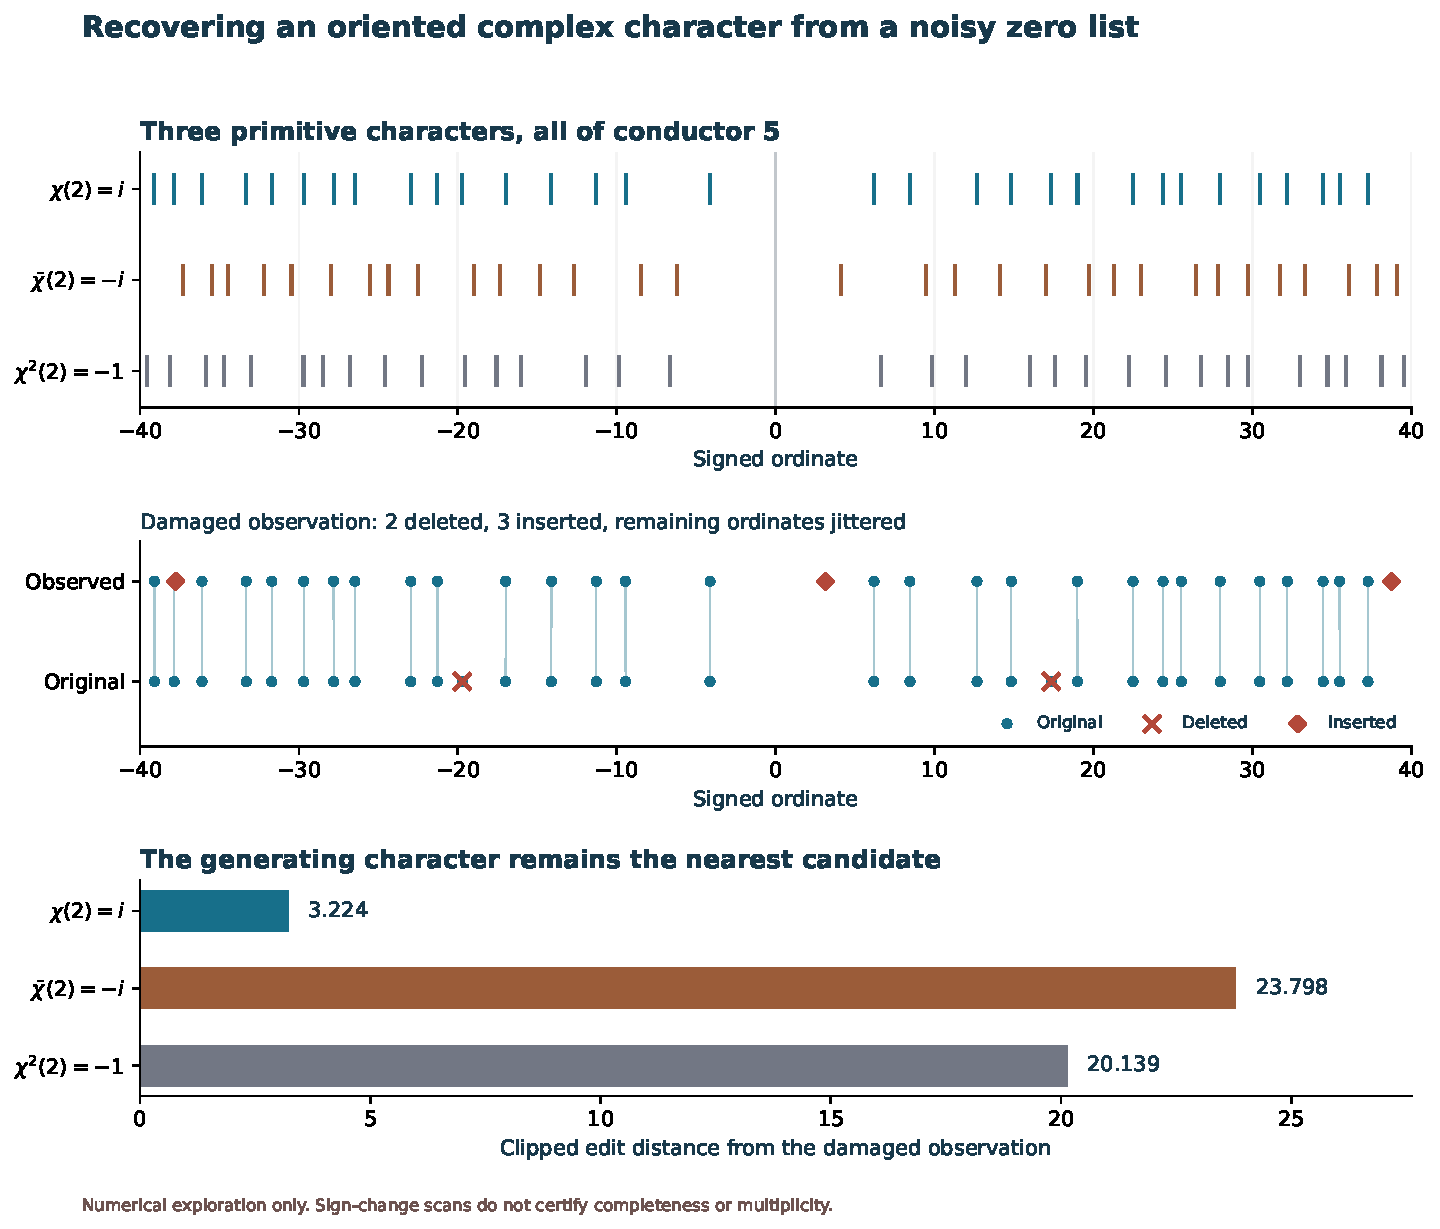
\includegraphics[width=\linewidth]{demo/complex_zero_lists.pdf}
\caption{Signed numerical ordinates for the three conductor-$5$
characters and the damaged observation. The quartic spectrum and
its reflection encode the conjugate orientation. The height-$40$
lists are numerical illustrations, not certified complete spectra.}
\end{figure}

This example is deliberately separated from the theorem's
certificate. A sign-change scan can miss an even-multiplicity zero
or several crossings in one mesh interval. Small residuals verify
the detected approximate roots but do not certify completeness or
multiplicity. Height $40$ is also far below the conservative
universal cutoff in Theorem~\ref{thm:main}. Thus the example
illustrates the observation model and the metric, not an application
of the universal theorem at that height.

\subsection{Checks of the quantitative implementation}

The script \texttt{code/verify\_constants.py} evaluates the specified
cutoff and the explicit tail bound at several conductor bounds,
checks the exact integer inequality $m^2\le3^{m/2}$ for the orders
used in the calculations, and checks the scalar inequalities
appearing in the angular argument. Its output is saved in
\texttt{data/constants.json}. The arguments in the text, rather
than this finite sample of numerical checks, prove the inequalities
over their complete ranges.


The supplied programs check the finite numerical inequalities used
in the constants, compute the metric by minimum-cost assignment, and
verify small exact rational examples against exhaustive matching.
They also illustrate an oriented complex-character spectrum and
specified corruptions. These checks exercise the data model and
constants; the proofs of the infinite analytic statements are the
arguments in this report.

The new theorem has not been formalized or checked by Lean. No Lean
source with unproved placeholders is presented as a formal proof.
The proof-assistant status of the upstream RH/Dirichlet-GRH theorem
and the status of this new human-readable theorem are separate.
The included formalization roadmap identifies the interfaces needed
for a future Lean development.

The main limitations are concrete. We do not assert an optimal
cutoff or an optimal corruption constant. We do not identify a
character from an arbitrary incomplete list without a bound on the
missing-data cost. We do not remove the conductor upper bound $Q$.
Finally, the theorem does not extend Dirichlet GRH to nonabelian
Artin or general automorphic $L$-functions.

\appendix
\section{What the archimedean-free support accomplishes}

It may appear surprising that the finite decoder does not need the
conductor or parity of the unknown character. There are three
distinct reasons. First, the standard conductor term in Weil's
formula is proportional to the frequency test at $0$; the support
near $\log p$ makes it exactly zero. Second, the parity-dependent
gamma contribution is positive and is uniformly at most $1/16$
after normalization, so it fits in a common decoding margin.
Third, the possible zeta pole contribution is also at most $1/16$
because the factor $\sinc(Hu/8)^2$ reduces the mass of the frequency
test to $O(1/H)$ while preserving its value $1$ at the selected
prime. The same reduction makes the spectral test both bounded and
Lipschitz with constants $O(\sqrt X/H)$; that is precisely what
turns arithmetic separation into an error budget growing linearly
with the observed height.

The compact B-spline envelope performs a different task. It confines
the arithmetic support to one prime and provides high-order decay
outside the observed zero window. Its order $m$ grows only as
$\log\log Q$. Keeping these roles separate explains why the proof
can permit both an arbitrary number of character phases and
incomplete observations without a zero-spacing assumption.

\clearpage
\addcontentsline{toc}{section}{References}
\begin{thebibliography}{99}
\raggedright
\bibitem{sernau} L. Sernau, with colleagues at Anthropic and Claude,
\emph{GRH for Dirichlet L-functions, in Lean 4},
\href{https://github.com/lsernau/grh-lean}{GitHub repository},
commit \texttt{72fead102f663d5c7a407964a13dc0cf9d977207}, 25 November 2026.
Inspected: \texttt{README.md}, \texttt{grh/GUIDE.md},
\texttt{grh/src/Statements.lean}, \texttt{grh/src/Main.lean}, and selected
\texttt{New/Reduction} files.
\bibitem{leancommunity} Lean FRO and Mathlib Initiative,
\emph{Lean verification of the Riemann Hypothesis}, 21 November 2026,
\url{https://leanprover-community.github.io/blog/posts/riemann-hypothesis/}.
\bibitem{rubinstein} M. Rubinstein,
\emph{Alp\"oge/Claude proof of the Generalized Riemann Hypothesis},
verification reports, including the shortened proof checked 26 November 2026,
\url{https://www.math.uwaterloo.ca/~mrubinst/alpoge_claude_grh/}.
\bibitem{proveit} V. Reshetnikov, \emph{ProveIt: Generalized Riemann
Hypothesis research collection}, snapshot
\texttt{4d7990202f9f106b2ffe8c209f073ad01d5e1987},
\url{https://github.com/VladimirReshetnikov/ProveIt/tree/main/Analysis/GeneralizedRiemannHypothesis}.
\bibitem{quadraticpacket} ProveIt research packet,
\emph{Quadratic characters from finitely many zeros; Sharp bounds for
positive dilation averages}, 26 November 2026,
\path{Analysis/GeneralizedRiemannHypothesis/docs/incoming/quadratic_spectra.zip}
at the snapshot in
\cite{proveit}. Theorems 3.1 and 3.3 and the second final research question.
\bibitem{wiki} Wikipedia contributors, \emph{Riemann hypothesis},
version inspected 26 November 2026,
\url{https://en.wikipedia.org/wiki/Riemann_hypothesis}.
\bibitem{banks} W. D. Banks, \emph{Comparing zeros of distinct Dirichlet
$L$-functions}, Publ. Math. Debrecen \textbf{106} (2025), 327--335;
\url{https://arxiv.org/abs/2302.07073}.
\bibitem{bach} E. Bach, \emph{Explicit bounds for primality testing and
related problems}, Math. Comp. \textbf{55} (1990), 355--380,
\url{https://doi.org/10.1090/S0025-5718-1990-1023756-8}.
\bibitem{lls} Y. Lamzouri, X. Li, and K. Soundararajan,
\emph{Conditional bounds for the least quadratic non-residue and
related problems}, Math. Comp. \textbf{84} (2015), 2391--2412,
\url{https://arxiv.org/abs/1309.3595}.
\bibitem{bmor} M. A. Bennett, G. Martin, K. O'Bryant, and A. Rechnitzer,
\emph{Counting zeros of Dirichlet $L$-functions}, Math. Comp.
\textbf{90} (2021), 1455--1482,
\url{https://doi.org/10.1090/mcom/3599}.
\bibitem{fordzaharescu} K. Ford and A. Zaharescu,
\emph{Unnormalized differences between zeros of $L$-functions},
Compos. Math. \textbf{151} (2015), 230--252,
\url{https://arxiv.org/abs/1305.2520}.
\end{thebibliography}
\end{document}
